\documentclass{tudelftposter}
\usepackage{graphicx}
\usepackage{subfigure}
\title{TI2716-B License plate recognition, Poster 1}

\addauthornote{tu}{Group 8, Delft University of Technology}

\addauthor[tu]{Yinghao Dai}
\addauthor[tu]{Yanna van der Vlugt}

\addfootimage(c:right column.center)[Delft Institute of Applied Mathematics]{tudelft}


\begin{document}

\section{Introduction}
We are working on a license plate recognizer, which can, as the name already suggests, recognize license plates on cars under certain conditions. In the following, we will take you through the steps we have taken so far, and briefly state our plan for next week. 

\section{License plate detection}
Of course we need to detect the license plates before being able to recognize their characters. As the Dutch license plates are yellow, we can detect them by color. Therefore, we created scatterplots of the different color values of the license plates, and compared them to those of cars and other (background) objects. The scatterplot of the $G$ (green) against the $B$ (blue) value can be found in figure \ref{greenblue}. Based on these plots, we created certain thresholds, which an object needs to satisfy in order to be classified as a license plate. The thresholds are also shown in figure \ref{greenblue}, as pink lines. 

\begin{figure}[h]
	\centering
	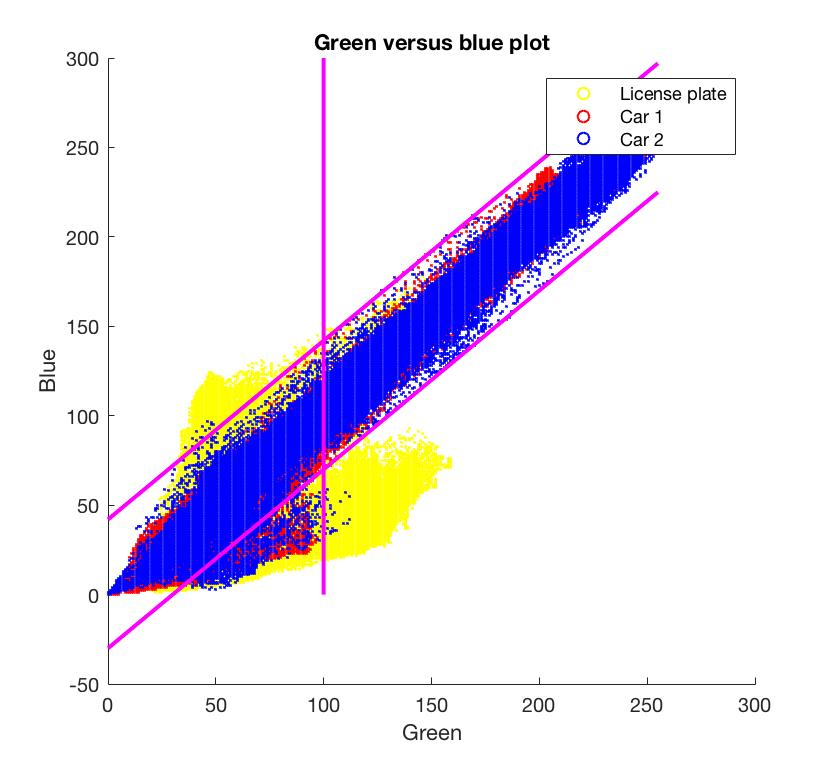
\includegraphics[width=995pt]{greenblueplot.jpg}
	\caption{Scatterplot of different objects ($G$ value against $B$ value).}
	\label{greenblue}
\end{figure}

\section{Standardization}
After having detected the license plate, we need to standardize it, to be able to properly recognize the characters. That means all plates need to be rotated, until they are horizontal. This process brings us from figure \ref{original} to \ref{rotate}. Unfortunately, we see that the license plate becomes hardly readable after this step, which made us decide to add an extra interpolation step, resulting in figure \ref{interpolate}. As a preparation step for the character recognition, we need to label the different characters on the license plate, which has been done in figure \ref{label}. 

\begin{figure}[h]
	\centering
	\subfigure[Original image]{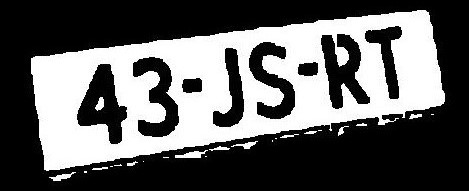
\includegraphics[width=500pt]{cropped.jpg}\label{original}}
	\subfigure[After rotation]{
\includegraphics[width=500pt]{rotatedwrong.jpg}\label{rotate}}
	\subfigure[After interpolation]{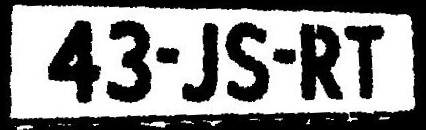
\includegraphics[width=500pt]{rotated.jpg}\label{interpolate}}
	\subfigure[After labeling]{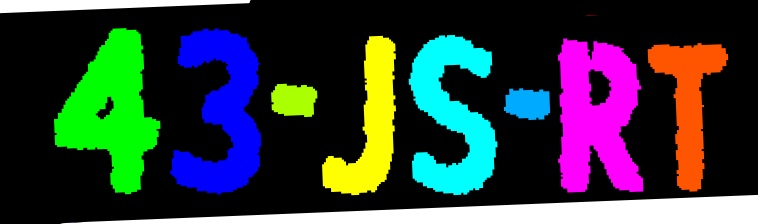
\includegraphics[width=500pt]{labeledletters.jpg}\label{label}}
	\caption{Process of standardizing a license plate.}
\end{figure}

\section{GUI}
For an application like ours, a graphical user interface (GUI) cannot be missing. A screenshot of the GUI is given in figure \ref{gui}. Note that the GUI has not yet been coupled to the back-end (since the latter is not yet able to correctly recognize the license plates). Hence, the ``recognized'' license plates in the screenshot are parts of dummy data. 

\begin{figure}[h]
	\centering
	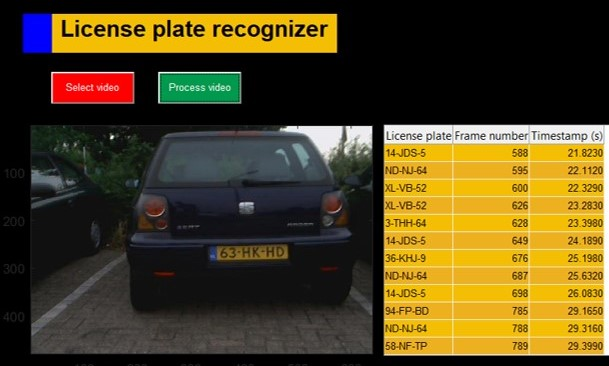
\includegraphics[width=1000pt]{gui.jpg}
	\caption{Graphical User Interface of our license plate recognizer.}
	\label{gui}
\end{figure}

\section{Focus for next week}
Next week, we are planning to improve the standardization process. Especially the rotation step still causes some problems at the moment. After this, we want to start recognizing the characters on the license plate. If we have time left, we can also start coupling the back-end to the GUI. 

\end{document}
%\experimentalblockright{%
%  SPAM:
%  Nulla malesuada porttitor diam. Donec felis erat, congue non, volutpat at,
%  tincidunt tristique, libero.}